\documentclass[notes]{beamer} % notes=only for notes, frames
\usetheme{metropolis}

\usepackage{amsmath,amsfonts}
\usepackage{graphicx}
\usepackage{hyperref}
\usepackage{tikz}
\usetikzlibrary {positioning}
\usetikzlibrary{arrows.meta}
\usetikzlibrary {automata}
\newcommand{\grad}{\nabla}

\input{sym}

\title[DRL for DL experts]{Deep Reinforcement Learning }
\author{Vikas Dhiman}

\begin{document}
\maketitle

%\begin{frame}
%  Prerequisites for knowing Reinforcement Learning
%  \begin{enumerate}
%    \item Linear algebra 
%    \item Probability
%    \item Python
%  \end{enumerate}
%
%  Prerequisites for knowing Deep Reinforcement Learning
%  \begin{enumerate}
%  \item Deep Learning
%  \end{enumerate}
%\end{frame}

\begin{frame}{BF Skinner's Reinforcement Learning for Pigeons}
  \centering
  \href{http://bfskinner.org/wp-content/uploads/2015/02/Operant_Conditioning.mp4}{Video}\\
  \includegraphics[width=0.45\linewidth]{media/pigeon-peck.png}%
  \includegraphics[width=0.45\linewidth]{media/pigeon-turn.png}
  \footnote{Image source:bfskinner.org}

\end{frame}

\note{
  \begin{enumerate}
  \item BF Skinner demonstrated that pigeons could learn to repeat an action
    that lead them to a particular reward.
    \cite[p15]{sutton2020reinforcement}
  \end{enumerate}
}

\begin{frame}{RL terminology}
  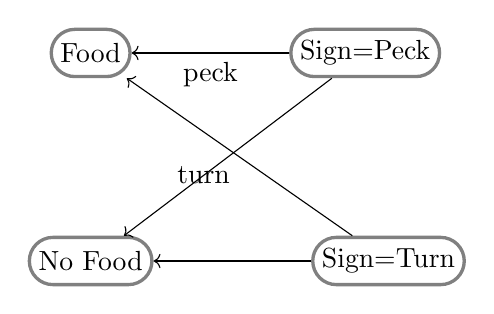
\begin{tikzpicture}[node distance=20mm,
    state/.style={
      % The shape:
      rectangle,minimum size=6mm,rounded corners=3mm,
      % Border
      very thick,draw=black!50
      }]
  \node (food) [state] {Food};
  \node (no-food) [state, below=of food] {No Food};
  \node (sign-peck) [state,right=of food] {Sign=Peck};
  \node (sign-turn) [state,right=of no-food] {Sign=Turn};
  \draw [->] (sign-peck) to [edge label=peck] (food);
  \draw [->] (sign-peck) to (no-food);
  \draw [->] (sign-turn) to [edge label=turn] (food);
  \draw [->] (sign-turn) to (no-food);
  \end{tikzpicture}
  \begin{description}
  \item[State ] ($\bfs_t \in \calS$) %Example: Sign is peck or turn. Food is
    %dispensed or not.
\pause
\item[Actions ] ($\bfa_t \in \calA$) %Example: To peck or to turn or no action.
  \pause
  \item[Transition probabilities]
    ($P(\bfs_{t+1}|\bfs_{t}, \bfa_t)$) %Example:
    %Probability of food dispensing if you peck when Sign-peck is shown.
    \pause
  \item[Rewards ] ($r_t \sim P(. | \bfs_t, \bfa_t) \in \bbR$) % Example: Food is high reward ($r_t = 100$).
    %food is zero-reward ($r_t = 0$).
    \pause
  \item[Policy ] $\pi(\bfs_t) \to \bfa_t$
  \item[Goal ] Maximize future reward $\sum_{k=t+1}^{T} r_k$
  \end{description}
\end{frame}
\note{
  State is the full description of the world at time $t$ that captures the
entire history. Example: in this example the state can be captured with two bits
$\bfs_t = [f_t; p_t]$, where $f_t \in \{0, 1\}$ describes a food or no food
state and $p_t \in \{0, 1\}$ describes the sign showing  peck or turn.
}

%\begin{frame}{Better state diagram}
%  \begin{tikzpicture}[node distance=20mm,
%    state/.style={
%      % The shape:
%      rectangle,minimum size=6mm,rounded corners=3mm,
%      % Border
%      very thick,draw=black!50
%    },
%    every to/.style={
%      thick,bend right
%    }
%    ]
%    \node (food-turn) [state] {Food/Sign=Turn};
%    \node (food-peck) [state, below=of food] {Food/Sign=Peck};
%    \node (no-food-turn) [state,right=of food] {NoFood/Sign=Turn};
%    \node (no-food-peck) [state,right=of no-food] {NoFood/Sign=Peck};
%    \draw [-Stealth](no-food-turn) to [edge label=turn] (food-turn);
%    \draw [-Stealth](no-food-peck) to [edge label=peck] (food-peck);
%    \draw [-Stealth](food-turn) to [edge label=eat] (no-food-turn);
%    \draw [-Stealth](food-peck) to [edge label=eat] (no-food-peck);
%    \draw [-Stealth](no-food-turn) to [edge label=?] (no-food-peck);
%    \draw [-Stealth](no-food-peck) to [edge label=?] (no-food-turn);
%    \draw [-Stealth] (no-food-turn.north) to [in=45,out=-45,loop,edge label'=peck] (no-food-turn.north);
%
%    \draw [-Stealth] (no-food-peck.south) to [in=135,out=-135,loop,edge label=turn] (no-food-peck.south);
%  \end{tikzpicture}
%  
%\end{frame}

\begin{frame}{Applications of RL}
  \centering
  \begin{columns}
    \column{1em}
    % Column 1
    \column{0.5\linewidth}
    \begin{minipage}{\linewidth}
      \includegraphics[width=0.9\linewidth]{./media/DQN-breakout.png}\\
      Atari games\cite{mnih2015human}
    \end{minipage}\\
    \pause
    \begin{minipage}{\linewidth}
    \includegraphics[width=0.9\linewidth]{./media/alphago-leesedol.png}\\
    Alpha Go\cite{silver2016mastering}
    \end{minipage}
    % Column 2
    \column{0.5\linewidth}
    \pause
    \begin{minipage}{\linewidth}
    \includegraphics[width=0.6\linewidth]{./media/recommender-systems.png}\\
    Recommender systems
    \end{minipage}\footnote{Img: towardsdatascience.com}
    \pause
    \begin{minipage}{\linewidth}
      \includegraphics[width=0.7\linewidth]{./media/autonomous-cars.jpeg}\\
      Autonomous cars
    \end{minipage}\footnote{Img:udacity.com}
  \end{columns}
\end{frame}

\begin{frame}{Exercise: Modeling the Breakout game}
  \centering
  \includegraphics[width=0.6\linewidth]{./media/DQN-breakout.png}
  \begin{enumerate}
  \item State space? 
  \item Action space? 
  \item Rewards?
  \end{enumerate}
\end{frame}


\begin{frame}{RL problem}
  \begin{description}
  \item[Discount factor ] $\gamma \in (0,1]$.
  \end{description}
  \begin{align*}
    \pi^*(.) = \arg~\max_{\pi} \bbE\left[\sum_{t=0}^{T}
      \gamma^{t} r_t \right]
   % \\
   % \text{such that } \bfs_{t+1}\sim P(.|\bfs_t, \pi(\bfs_t))\, \forall t \in [k, \infty) \\
   % \text{ and } \bfs_0 \sim p_0(.) 
  \end{align*}
\end{frame}

\begin{frame}{Value Function}
  \begin{align*}
    V_\pi(\bfs_k) &= \bbE\left[\sum_{t=k}^{T}
    \gamma^{t-k} r_t \middle| \bfs_k\right]
    %\\
    %\text{such that }& \bfs_{t+1}\sim P(.|\bfs_t, \pi(\bfs_t)) \forall t \in [k, \infty)\\
  \end{align*}
\end{frame}

\begin{frame}{Action Value Function}
  \begin{align*}
    V_\pi(\bfs_k) &= \bbE\left[\sum_{t=k}^{T}
                    \gamma^{t-k} r_t \middle| \bfs_k\right] \\
    Q_\pi(\bfs_k, \bfa_k) &= \bbE\left[\sum_{t=k+1}^{T}
                    \gamma^{t-k-1} r_t \middle| \bfs_k, \bfa_k \right]
    %\\
    %\text{such that }& \bfs_{t+1}\sim P(.|\bfs_t, \pi(\bfs_t)) \forall t \in [k, \infty) \\
  \end{align*}
\end{frame}

\begin{frame}{Advantage Function}
  \begin{align*}
    V_\pi(\bfs_k) &= \bbE\left[\sum_{t=k}^{T}
                    \gamma^{t-k} r_t \middle| \bfs_k\right] \\
    Q_\pi(\bfs_k, \bfa_k) &= \bbE\left[\sum_{t=k+1}^{T}
                            \gamma^{t-k-1} r_t \middle| \bfs_k, \bfa_k \right]
    \\
    A_\pi(\bfs_k, \bfa_k) &= Q_\pi(\bfs_k, \bfa_k) - V_\pi(\bfs_k)
                          % \\
                          % \text{such that }& \bfs_{t+1}\sim P(.|\bfs_t, \pi(\bfs_t)) \forall t \in [k, \infty) \\
  \end{align*}
\end{frame}

\begin{frame}{Bellman Equation}
  \begin{align*}
    V_*(\bfs_k) &= \bbE\left[\sum_{t=k}^{T}
                    \gamma^{t-k} r_t \middle| \bfs_k\right] \\
    Q_*(\bfs_k, \bfa_k) &= \bbE\left[\sum_{t=k+1}^{T}
                            \gamma^{t-k-1} r_t \middle| \bfs_k, \bfa_k \right]
                          \\
    &= \bbE[r_k + \gamma V_*(\bfs_{k+1})] \\
    &= \bbE[r_k + \gamma \max_{\bfa'} Q_*(\bfs_{k+1}, \bfa') | \bfs_k, \bfa_k]
                          % \\
                          % \text{such that }& \bfs_{t+1}\sim P(.|\bfs_t, \pi(\bfs_t)) \forall t \in [k, \infty) \\
  \end{align*}
\end{frame}

\begin{frame}{DQN (2013): Bellman equation as a loss function}
  \tiny
  \begin{align*}
    L(\theta) &= \bbE_{(s,a,r,s') \sim U(D)} \left[\left(
    r + \gamma \max_{a'} Q(s', a'; \theta^-) - Q(s, a; \theta)\right)^2\right]
    \\
    \grad_\theta L(\theta) & = \bbE_{(s,a,r,s') \sim U(D)} \left[
    -\grad_\theta Q(s, a; \theta) \left(r + \gamma \max_{a'} Q(s', a'; \theta^-) - Q(s, a; \theta)\right)\right]
  \end{align*}
  \includegraphics[width=0.7\linewidth]{./media/DQN-arch.png}
\end{frame}

\begin{frame}{Other design considerations}
  \begin{enumerate}
  \item Exploration vs exploitation trade-off
  \item Off-policy vs on-policy learning
  \end{enumerate}
\end{frame}

\begin{frame}{DDPG (2015) : Deep deterministic Policy gradients}
  \tiny
  \begin{align*}
    \grad_\phi L(\phi) &= -\bbE_{(s, a, r, s') \sim U(D)}[\grad_a Q(s, a; \theta)\grad_\phi \pi(s; \phi)]
    \\
    \grad_\theta L(\theta) & = \bbE_{(s,a,r,s') \sim U(D)} \left[
                             -\grad_\theta Q(s, \pi(s; \theta); \theta) \left(r + \gamma \max_{a'} Q(s', \pi(s'; \phi^-); \theta^-) - Q(s, \pi(s; \phi); \theta)\right)\right]
  \end{align*}
  \includegraphics[width=0.3\linewidth]{./media/cheetah.png}
\end{frame}

\begin{frame}{A3C (2016): Async. Advantage Actor Critic}
    \includegraphics[width=0.5\linewidth]{./media/A3C.png}\footnote{Img:towardsdatascience.com}

    {\tiny
    \begin{align*}
      \grad_\theta L_V(\theta) &= \bbE_{(s,a,r,s') \sim U(D)} \left[
                                 -\grad_\theta V(s;\theta_v) (r +  \gamma V(s'; \theta_V^-)  - V(s; \theta_V)) \right]
      \\
      \grad_\phi L_\pi(\phi) &= - \bbE_{(s,a,r,s') \sim U(D)} \left[\grad_\phi \log\pi(a|s;\phi)A(s, a;\theta) \right]
    \end{align*}
    }
\end{frame}

%\begin{frame}{SAC (2018): Soft actor critic}
%  \begin{align*}
%    L_V(\theta) = \bbE_{(s,a,r,s') \sim U(D)}\left[ \left(
%    V(s;\theta) - \bbE_{a' \sim \pi(.;\phi)}[Q(s, a') - \log \pi(a'|s; \phi)]
%    \right)^2 \right]
%  \end{align*}
%\end{frame}

\begin{frame}
  \href{https://vikasdhiman.info/safe-autonomous-nav-talk-sep2022/\#/other-work-video}{My work}
\end{frame}

\begin{frame}{References}
  \footnotesize
    \bibliography{main}
    \bibliographystyle{plain}
\end{frame}
\end{document}
